\documentclass{article}

\usepackage[utf8]{inputenc}
\usepackage{graphicx}
\usepackage{amsmath}
\usepackage[letterpaper, portrait, margin=1in]{geometry}
\usepackage{booktabs}

\title{Biomaterials HW 3}
\author{Nikhil Menon}
\date{September 28th, 2016}

\begin{document}

\maketitle

1. \begin{figure}[h]
  \centering
 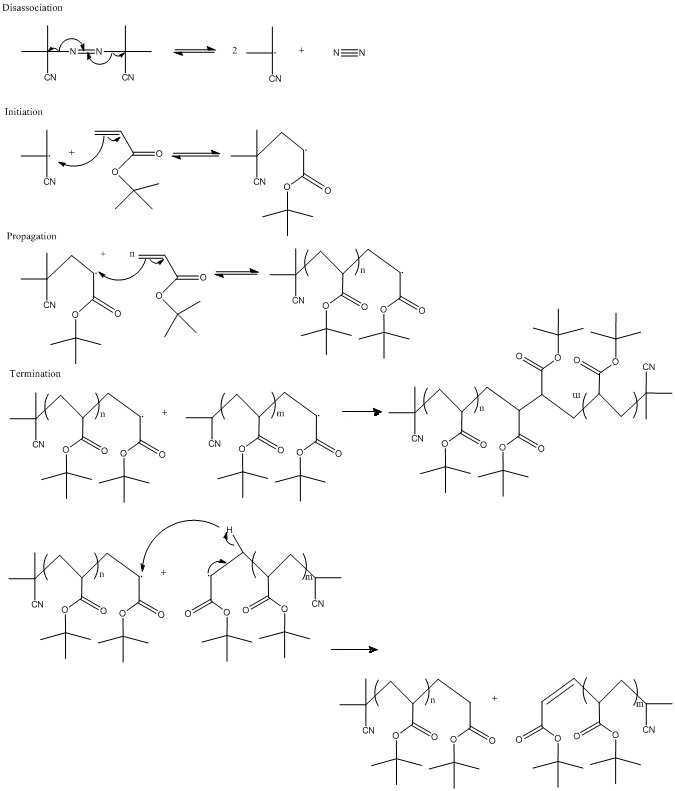
\includegraphics[scale=0.8]{P1a.jpg}
\end{figure}
\begin{figure}[h]
  \centering
 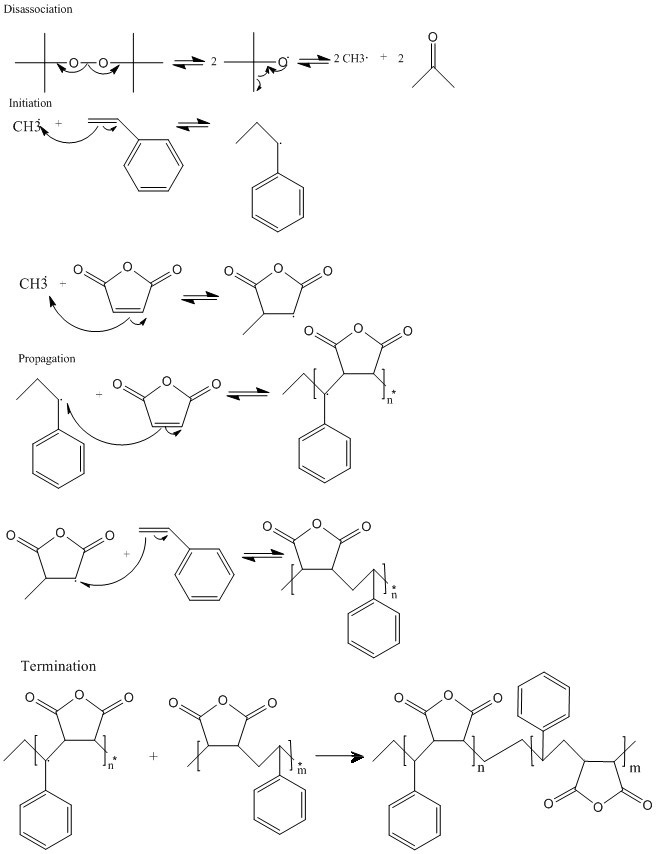
\includegraphics[scale=0.7]{P1b.jpg}
\end{figure}

2a. From the problem, we know that
$$k_d=4.47x10^{-6} s^{-1},\frac{k_p^2}{k_t}=1x10^{-2} mol^{-1}/s, f=0.4$$

First, convert the concentrations of the two chemicals to molar concentrations (Molar mass of methyl methacrylate is 100.14 g/mol and molar mass for benzoyl peroxide is 242.23 g/mol)
$$[benzoyl\hspace{1mm} peroxide]=[M]=0.9988 M$$
$$[methyl\hspace{1mm} methacrylate]=[I]=0.00411 M$$

Then, since the concentration of I changes over time,
$$-\frac{d[I]}{dt}=2fk_df[I]_0$$

which, after integrating, becomes
$$[I]=[I]_0e^{-2fk_dt}$$

The steady state rate of polymerization is
$$R_p=k_p\left(\frac{fk_d}{k_t}\right)^{1/2}[M][I]^{1/2}$$

which, after substituting the previous formula, becomes
$$-\frac{d[M]}{dt}=k_p\left(\frac{fk_d}{k_t}\right)^{1/2}[M]\left([I]_0e^{-2fk_dt}\right)^{1/2}$$

which, after integrating, becomes
$$-ln\frac{[M]}{[M]_0}=k_p\left(\frac{fk_d}{k_t}\right)^{1/2}[I]_0^{1/2}\left(\frac{e^{-fk_dt}}{-fk_d}\right)$$

Since $[M]/[M]_0=0.5$, we can solve for t to get
$$t=24.7 hours$$

2b. Then, combining the formula
$$x_n=\frac{k_p[M]}{(1+q)k_t^{0.5}(\frac{R_i}{2})^{0.5}},q=1$$

and the formula
$$R_i=2fk_d[I]$$

gives
$$x_n=\frac{k_p[M]}{(2k_t^{0.5}(fk_d[I])^{0.5}}$$

We can also substitute the formula for [I] in terms of $[I]_0$ that we found earlier to get
$$x_n=\frac{k_p[M]}{(2k_t^{0.5}(fk_d[I]_0e^{-2fk_dt})^{0.5}}=739$$


3a. \begin{figure}[!h]
  \centering
 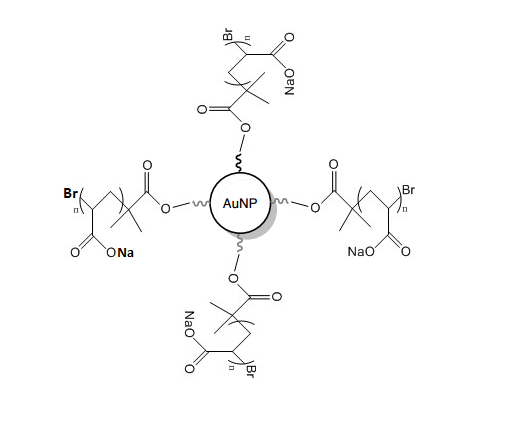
\includegraphics[scale=0.5]{P3a.png}
\end{figure}
\vspace{50mm}

3b.
 \begin{figure}[h]
  \centering
 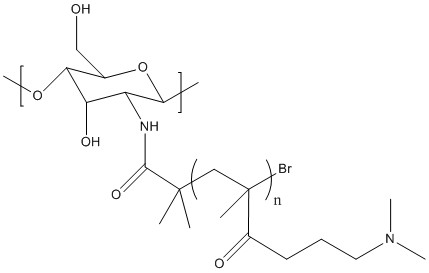
\includegraphics[scale=0.7]{P3b.jpg}
\end{figure}

\end{document}